\paragraph{Chiseling}

The \textbf{chiseling} procedure has two parts to it.
First, with one hand a chisel has to be chosen.
Users have a choice between a small, medium, large and extra large chisel to perform the procedure.
With the other hand, users then have to pick up the hammer.
Since this procedure requires users to hold two surgical instruments at the same time, this procedure can get cumbersome.
However, users can easily avoid this by placing the instruments on the operating table in the middle of the OT and repositioning afterwards (Figure \ref{fig::ChiselPrepare}).

\begin{figure}[ht]
    \centering
    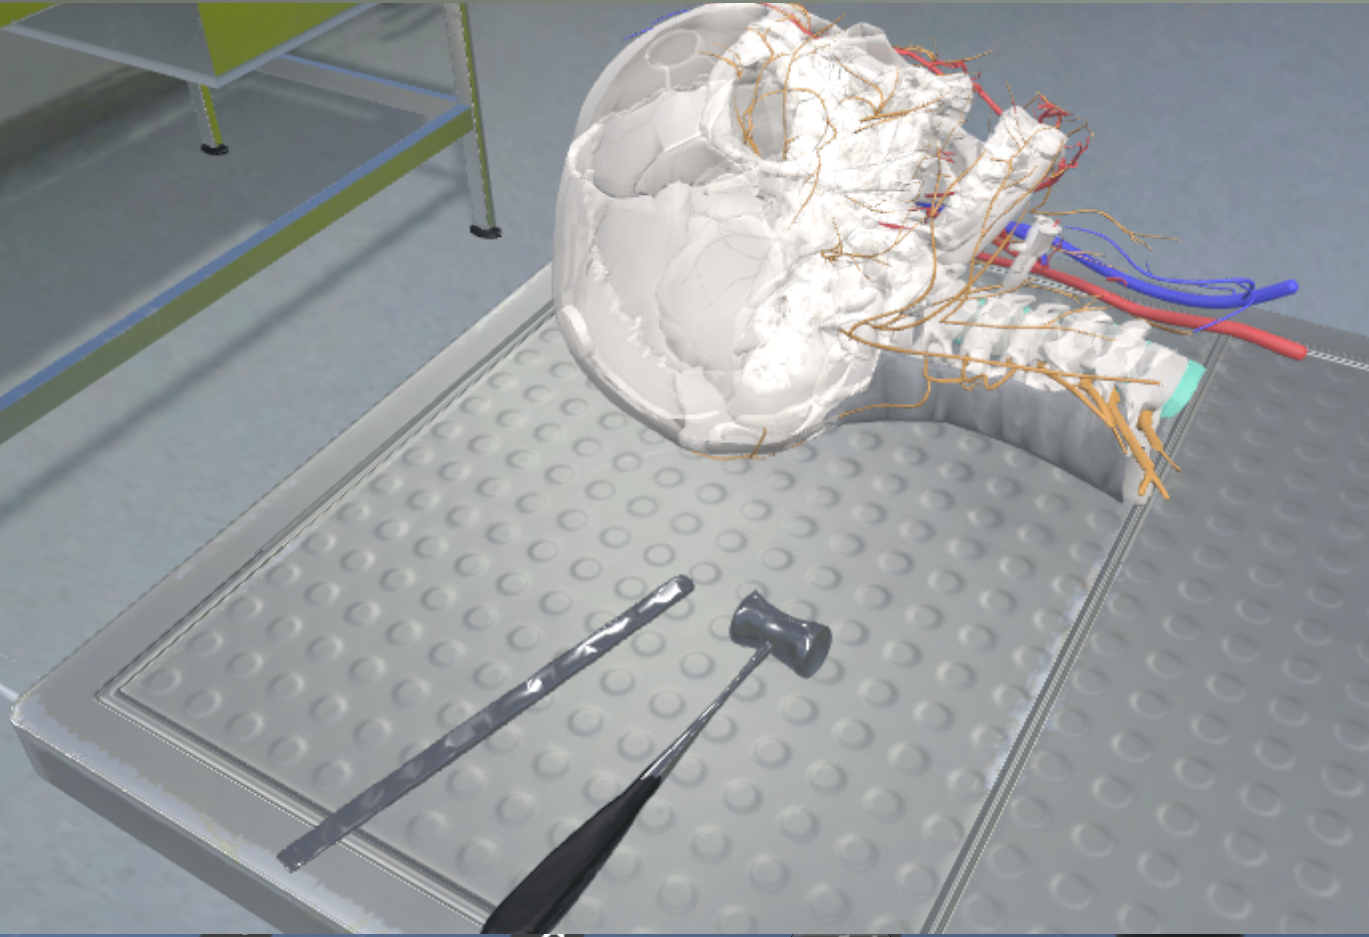
\includegraphics[width=\linewidth]{images/implementation/features/procedures/chisel_prepare.png}
    \caption{\label{fig::ChiselPrepare}The user prepares for the chiseling procedure by placing the instruments on the OT where the patient is located.
    indicators with the hammer in the other hand to perform the procedure.}
\end{figure}

When users have the perfect viewpoint, they can take up both instruments once again and start the procedure.
By pressing the indicate button on the hand where the chisel is located, rectangular indications at the top and bottom end of the chisel are shown to the user.
While these indications are active, the user has to perform a hammering motion with the hand holding the hammer.

\begin{figure}[ht]
    \centering
    \begin{minipage}{.5\textwidth}
      \centering
      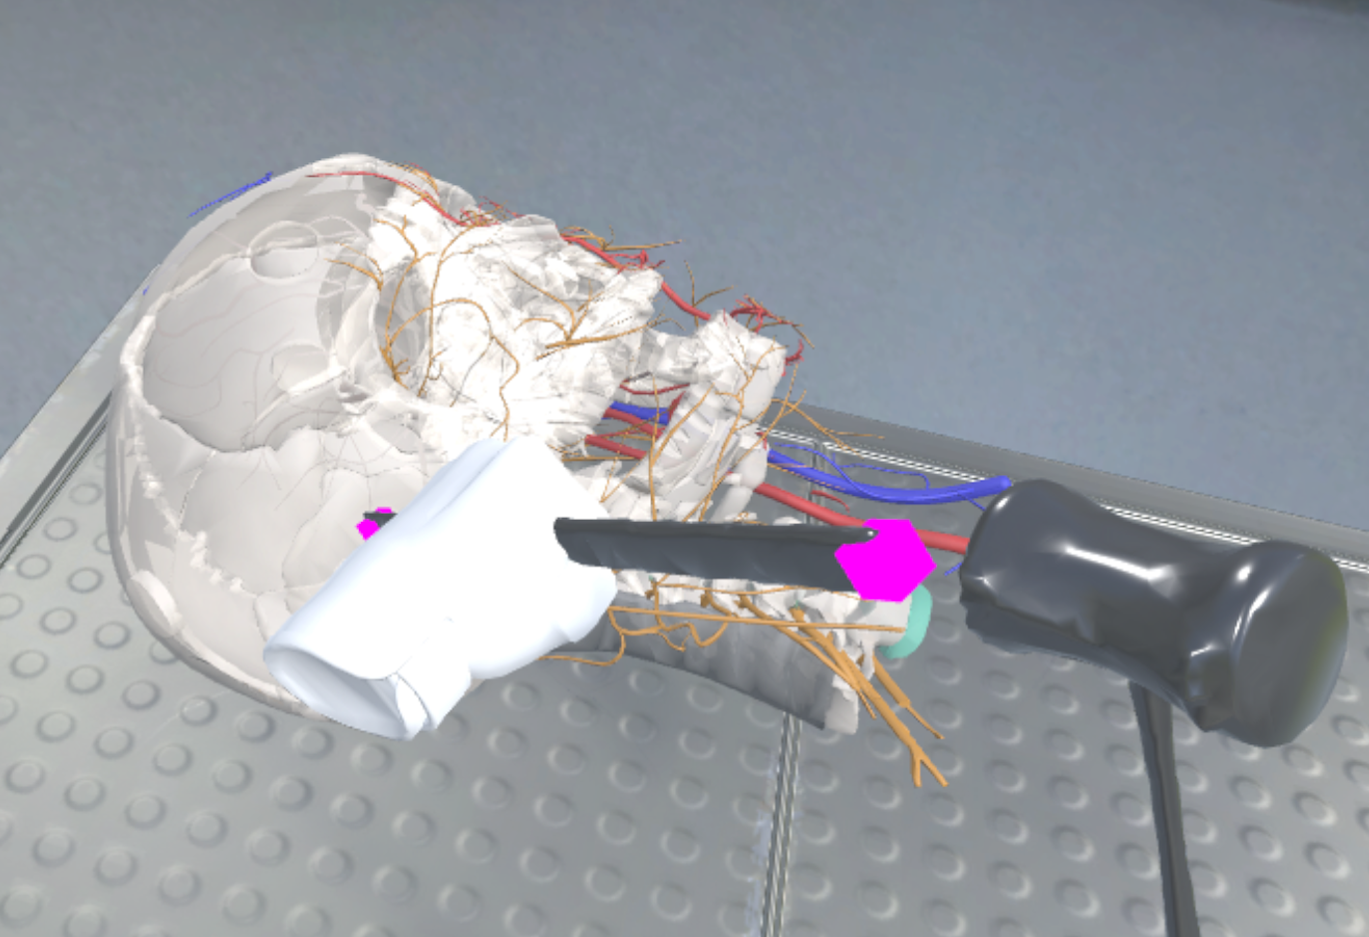
\includegraphics[width=0.99\linewidth]{images/implementation/features/procedures/chisel_1.png}
    \end{minipage}%
    \begin{minipage}{.5\textwidth}
      \centering
      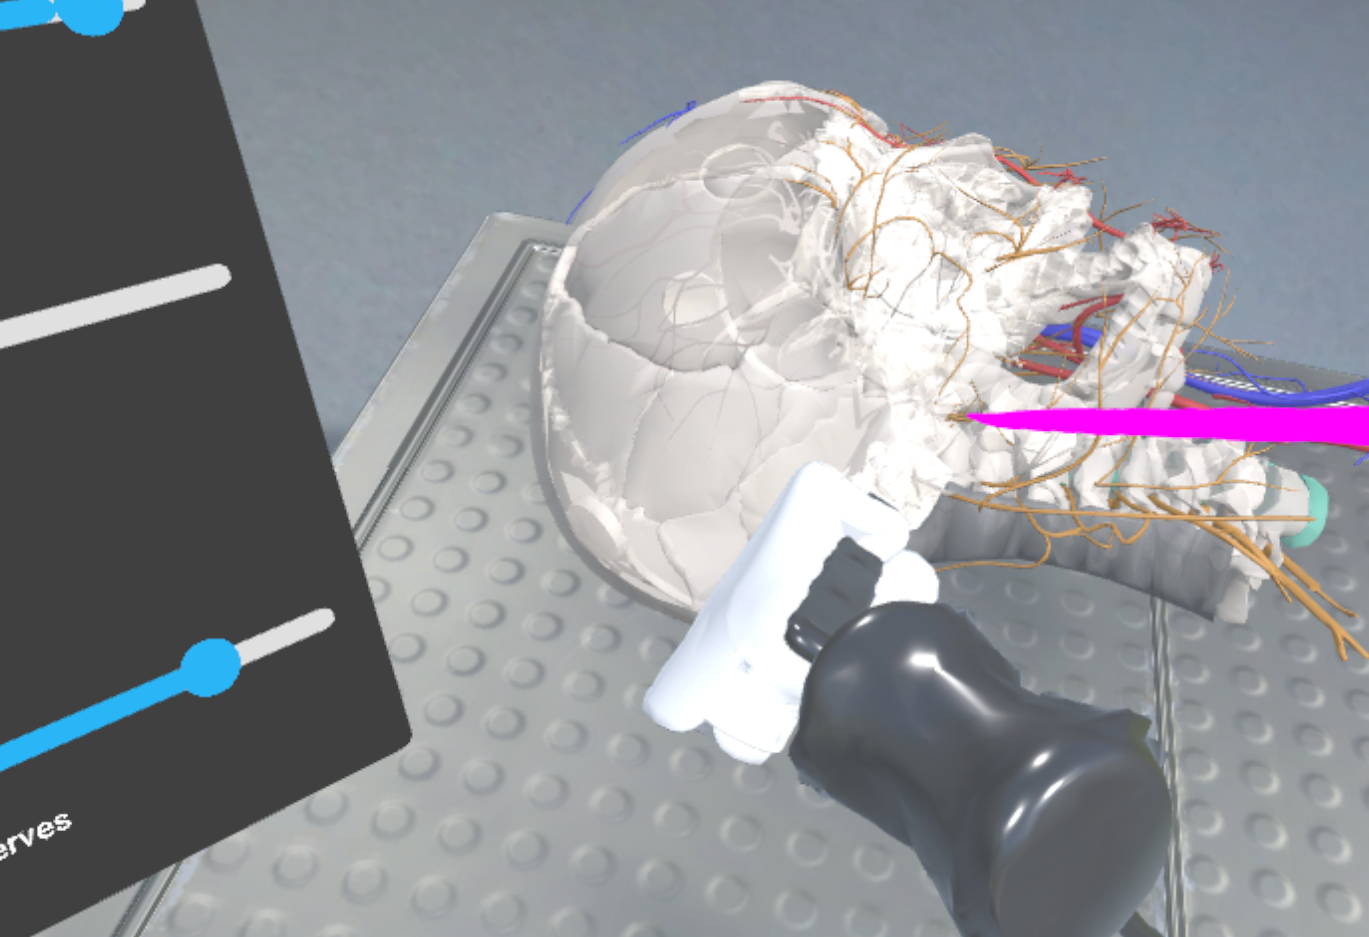
\includegraphics[width=0.99\linewidth]{images/implementation/features/procedures/chisel_2.png}
    \end{minipage}
    \caption{\label{fig::ChiselProcedure}Process of the chiseling procedure. Left: The users uses the indicate action with his left hand in preparation for the procedure. Right: After hammering on the indication on the chisel, the procedure has been performed and a step is generated.}
\end{figure}

When they hit the rectangular indicators located on the chisel, the chiseling procedure step is added to the project case in form of a modified copy of the hold chisel (Figure \ref{fig::ChiselProcedure}).
Here, information about the performed step is also included in the form of chisel size used for the procedure. 